\chapter{Theory}
\label{chap:theory}

\section{Sobel operator}
\label{sec:Sobel}
\paragraph*{}
The Sobel operator can be used to calculate the gradients in the image intensity and thus emphasizes the edges in a given image. The Sobel operator is defined as a $3~x~3$ matrix (equation \ref{eq:sobel_calc}) acting as a filter that is convoluted with the pictures pixels as it is moved along the x and y directions of the image.

\begin{equation}
\begin{array}{cc}
Gx = \left[ 
\begin{array}{ccc}
	-1 & 0 & 1\\
    -2 & 0 & 2\\
    -1 & 0 & 1\\
\end{array} \right] &
Gy = \left[ 
\begin{array}{ccc}
	1 & 2 & 1\\
    0 & 0 & 0\\
    -1 & -2 & -1\\
\end{array}
\right]
\end{array}
\label{eq:sobel_calc}
\end{equation}\\

\paragraph*{}
If a edge detection should be preformed on a $8~x~6$ image as illustrated in figure \ref{fig:pic_matrix} the steps would be to convolute the Sobel matricies $G_x$ and $G_y$ with the image pixels. If calculating the gray area in figure \ref{fig:pic_matrix} the result for green pixel ($A10$) would be given from equations \ref{eq:sobel_calc1} and \ref{eq:sobel_abs}.  

\begin{equation}
\begin{array}{c}
G_x = \left[ 
\begin{array}{ccc}
	-1\cdot A1 & 0\cdot A2 & 1\cdot A3\\
    -2\cdot A9 & 0\cdot A10 & 2\cdot A11\\
    -1\cdot A17 & 0\cdot A18 & 1\cdot A19\\
\end{array} \right] \\
\\
G_y = \left[ 
\begin{array}{ccc}
	1\cdot A1 & 2\cdot A2 & 1\cdot A3\\
    0\cdot A9 & 0\cdot A10 & 0\cdot A11\\
    -1\cdot A17 & -2\cdot A18 & -2\cdot A19\\
\end{array}
\right]
\end{array}
\label{eq:sobel_calc1}
\end{equation}\\

\begin{equation}
	A10=\vert G_x\vert + \vert G_y\vert
	\label{eq:sobel_abs}
\end{equation}
 
\begin{figure}[H]
	\centering
	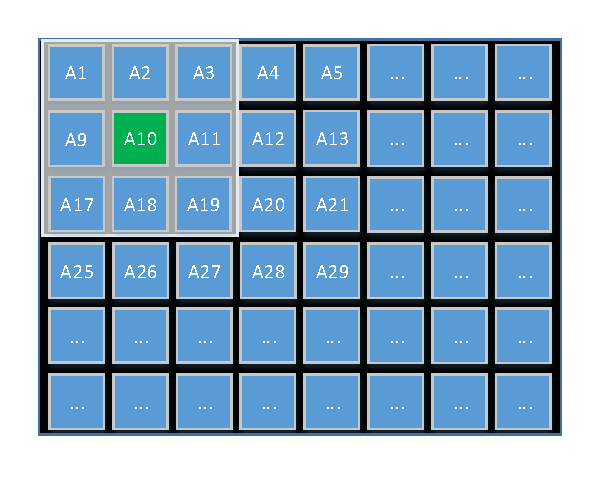
\includegraphics[width=0.5 \textwidth]{picture_example.pdf}
	\caption{Example of sobel matrix calculation}
	\label{fig:pic_matrix}
\end{figure}

\subsection{Border conditions}
\paragraph*{}
Since the Sobel operator is a $3~x~3$ matrix then performing Sobel operation on a pictures border pixel i problematic since the top/bottom row and left/right columns is outside the picture see figure \ref{fig:pic_matrix_border}. There is a couple of ways to handle this. One is to skip calculation of the border which result in a picture of $n-2~x~m-2$ calculated pixels and a untouched border. 

\begin{figure}[H]
	\centering
	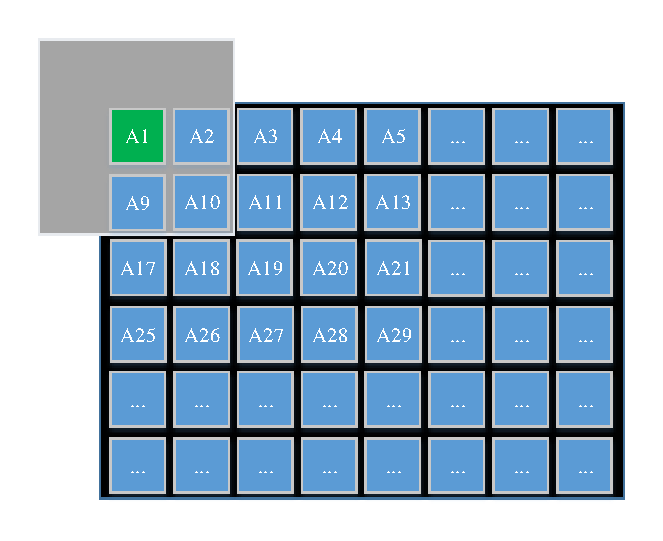
\includegraphics[width=0.5 \textwidth]{picture_example_border.pdf}
	\caption{Example of sobel matrix calculation at borders}
	\label{fig:pic_matrix_border}
\end{figure}

\paragraph*{}
A better and quite simple way to deal with the boarder problem is to make an imaginary or fictive border on the picture. This  can be done by coping the border pixels at the moment they are needed for calculation so that the border pixels give an extra border. The principle is illustrated in figure \ref{fig:pic_matrix_exBorder}.

\begin{figure}[H]
	\centering
	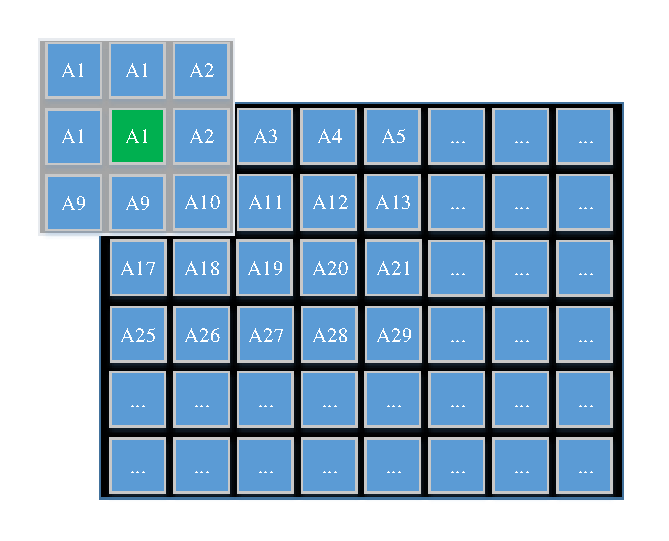
\includegraphics[width=0.5 \textwidth]{picture_example_exBorder.pdf}
	\caption{Example of sobel matrix calculation at borders}
	\label{fig:pic_matrix_exBorder}
\end{figure}  

\subsection{Dynamic range and normalization...}
\paragraph*{}

\section{Accelerator design} 
\label{sec:AccDesign}
\paragraph*{}
This section describes the design of the accelerator and explain how the pixel data is handled when travelling from external memory to the accelerator and back to external memory. 
Because each memory transaction involves two pixels (16bit data width). The proposed design of the accelerator, will process two pixels in parallel, this will increase the throughput without increasing the clock rate. At the same time it also simplifies the data handling, since the accelerator does not need to distinguish between which pixel to process (lower byte or upper byte). The drawback of this parallel approach is that the combinatorial logic that performs the Sobel operation, will be twice as big.

\paragraph*{}
As seen in the previous section \ref{sec:Sobel}, any given pixel, in the output image of the Sobel operator, is a function of the surrounding eight pixels in the input image. This requires that the accelerator is having access to these surrounding pixels, in order to evaluate the Sobel operator. Instead of reading the entire neighborhood from the external RAM, for every single pixel, an obvious improvement is to use a sliding window technique, and thereby reducing the number of memory transactions. If two pixel are to be processed in parallel, a 3x4 sliding window is required. But since the two convolution kernels stretches over three memory addresses, the width of the sliding window must be increased by one pixel, giving a total of 3x5 pixels. This is visualized in figure \ref{fig:shift_register}(a), which shows the two overlapping convolution kernels \emph{(A and B)} and the three memory location they span. \\
Figure \ref{fig:shift_register}(b) shows the proposed sliding window and illustrates how incoming pixels are shifted from right to left.

\begin{figure}[H]
	\centering
	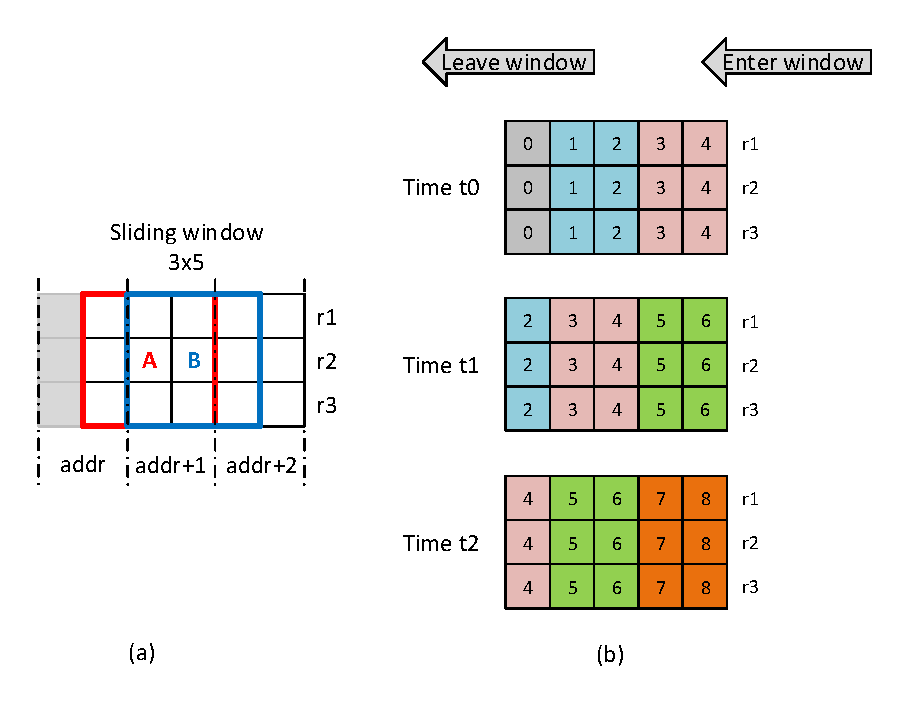
\includegraphics[width=0.9 \textwidth]{SlidingWindow.pdf}
	\caption{3x5 pixel sliding window}
	\label{fig:shift_register}
\end{figure}

\paragraph*{}
A block diagram showing the internal architecture of the accelerator is seen in figure \ref{fig:AccBlockDiagram}. The figure shows how data will flow from memory, over the sliding window through the Sobel operator and back to the memory again. A few control signals to control the memory and sliding window are also depicted in the figure. 

\begin{figure}[H]
	\centering
	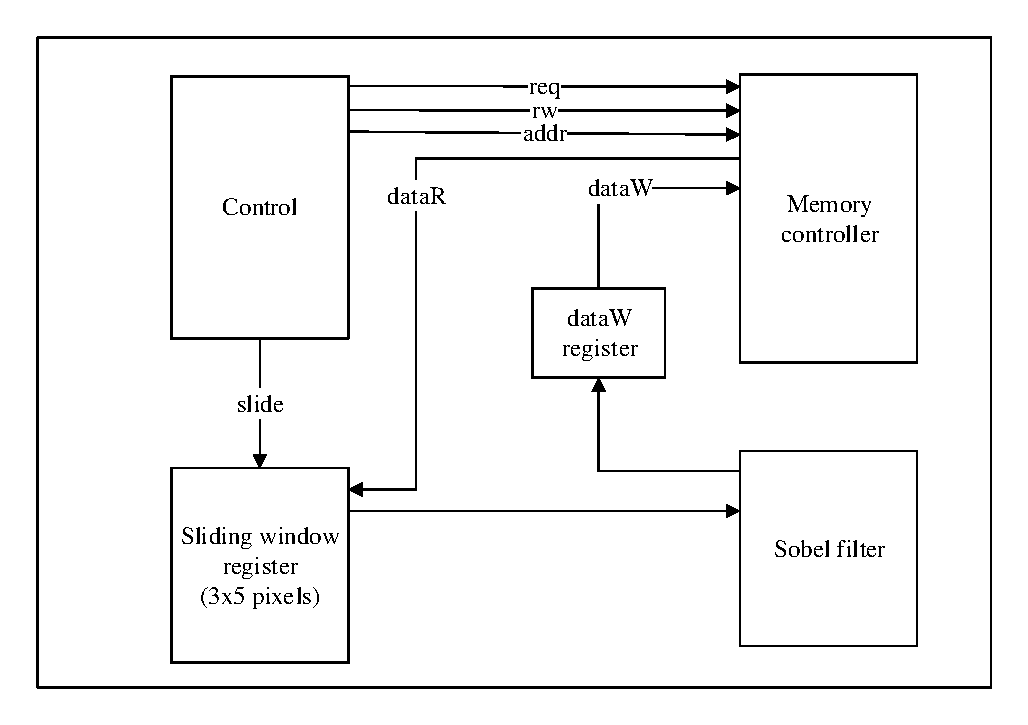
\includegraphics[width=1.0 \textwidth]{Block_diagram_overview.pdf}
	\caption{Internal architecture of the accelerator}
	\label{fig:AccBlockDiagram}
\end{figure}

\paragraph*{}
From the architecture seen in figure \ref{fig:AccBlockDiagram} along with sliding window from figure \ref{fig:shift_register} it is possible to give an initial estimate of the attainable throughput of the accelerator. For each processed pixel pair, the accelerator is required to perform three memory reads and one memory write. Because the memory controller needs to setup the address prior to reading and writing, two extra cycles are to be expected, giving a total of six clock cycles per pixel pair.
With a clock frequency of 12.5 MHz (maximum when the memory is operated in asynchronous mode) this gives a throughput of approximately 4.1M pixel/sec.
\paragraph*{}
ToDo - Estimating ressource usage ...

\paragraph*{}
Figure \ref{fig:ASM_HW} shows a complete ASMD diagram of the proposed design, that illustrates the operation of the sliding window and details about the image border handling. The ASMD diagram consist of 9 states (\emph{idle, startRow, readSetup, readCenter, readAbove, readBelow, calculateFilter, writeData and doneImage}).
In the \emph{idle} state the accelerator is waiting for the start signal to appear. Once the start signal is detected, the state is changed to \emph{startRow}, in which the current address is initialized to the start of the current image row before entering the next state \emph{readSetup}. In the state \emph{readSetup} the reading of the current address is prepared, this state also handles the sliding of the window as well as the special case for the left and right images borders. The state \emph{readCenter} will put the the newly read data into the sliding window and prepare the reading of data located one row above the current position. In case of first row the top image border is handled by reading the current position once more. The state \emph{readAbove} is almost identical to \emph{readCenter}, the difference is that it will prepare the reading of data one row below the current position and that it is handling the bottom image border. The state \emph{calculateFilter} is performing the Sobel operation and moves the result into a register. The \emph{writeData} state will write the content of the result register to the output image. From the \emph{writeData} state it is possible to enter one of three states. 1)\emph{startRow} in case the end of a row is reached. 2)\emph{doneImage} if the entire image has been processed and 3)\emph{readSetup} in the normal case.
The \emph{writeData} state will increment the current position and current row accordingly. The final state \emph{doneImage} will wait until the start signal is de-asserted before the FSM is returned to the \emph{idle} state.

\begin{figure}[H]
	\centering
	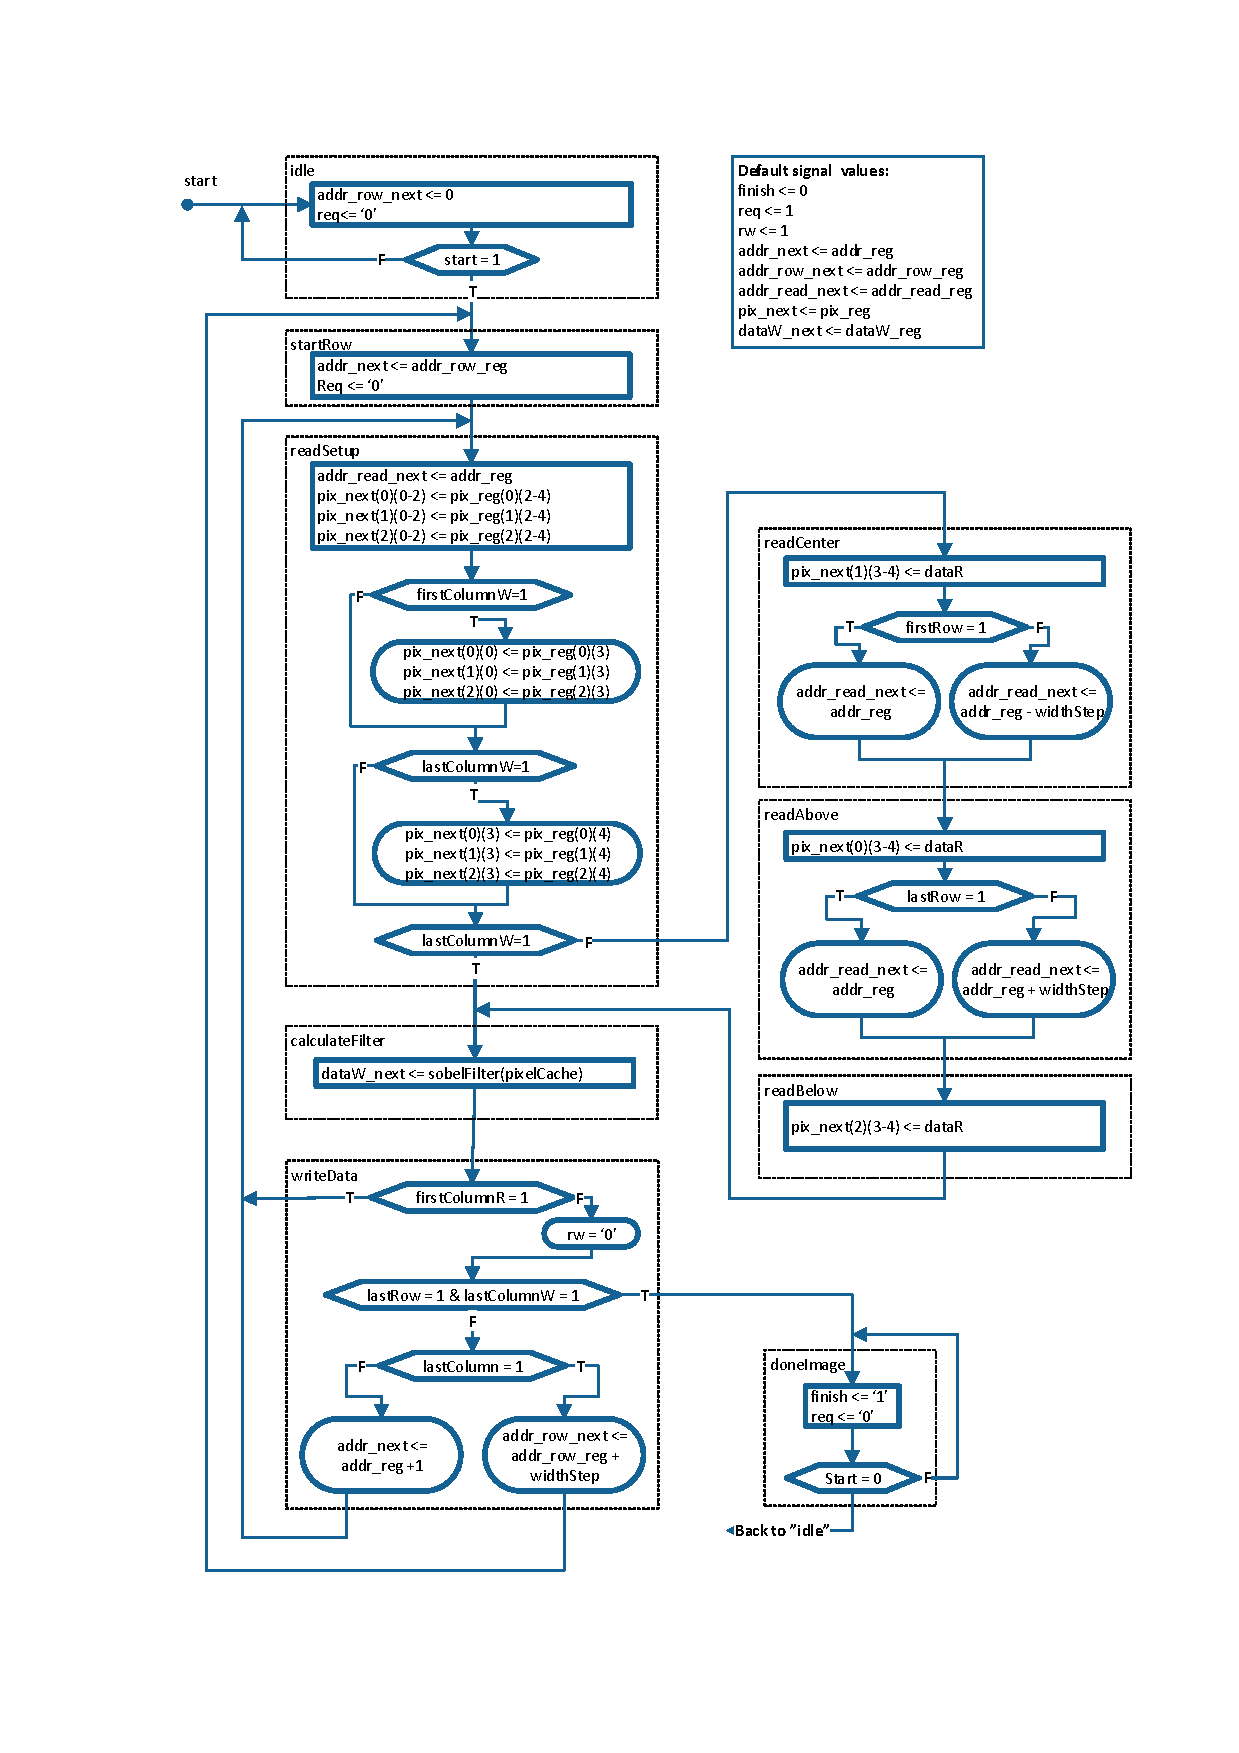
\includegraphics[width=1 \textwidth]{ASM_HWacc.pdf}
	\caption{ASMD chart for the edge detector hardware accelerator}
	\label{fig:ASM_HW}
\end{figure}

\section{Design optimization}
\label{sec:Optimization}
\subsection*{Removing superfluos reads}
\label{sec:memaccess}
\paragraph*{}
Even though the sliding window technique reduces the required memory transactions, the design presented in section \ref{sec:AccDesign}, still need to read every single pixel three times. This is caused by the fact that each row will need data from the row above and below the current position. Since access to the external memory is the main bottleneck in terms of achieving a high throughput, it is desirable to only read the pixel data once. By employing even more caching of data this is indeed possible. Figure \ref{fig:ScanlineBuffers} shows a caching scheme that will assure that data from three consecutive rows are available and ready to enter the sliding window. The cache operates as a delay-line buffer with one tap and contains two full scanlines. Whenever a pixel is read from the external memory it is pushed into one end of the scanline buffer and the tap and end of the delay line buffer will hold pixel data from the two rows just above the pixel being pushed into  scanline buffer. In practise the scanline buffer is implemented as a ring buffer with two pointers addressing the middle-tap and the end position.

\begin{figure}[H]
	\centering
	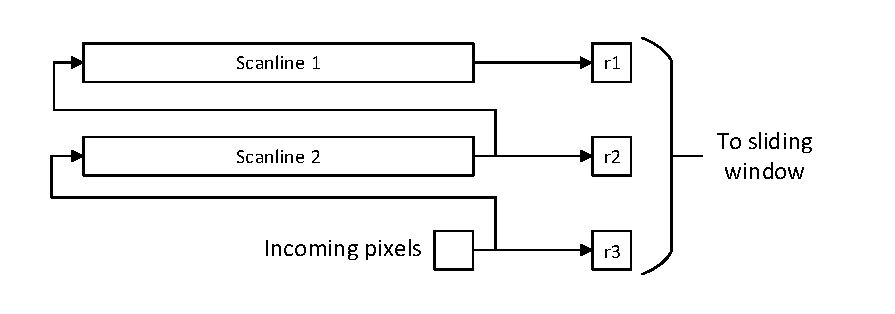
\includegraphics[width=0.9 \textwidth]{ScanlineBuffers.pdf}
	\caption{Scanline buffering of pixel data.}
	\label{fig:ScanlineBuffers}
\end{figure}
\paragraph*{}

The scanline buffer can be implemented as either distributed RAM (using LUT's) or via the block RAM, which is present on most modern FPGA's. Block RAM is usually preferred when larger memories are needed, since the distributed RAM requires many FPGA ressources. The Xilinx Spartan6 chip, used in this assignment, has a true dual ported Block RAM, which is capable of both reading and writting to RAM in one single clock cycle.
\cite{Xilinx:UG383}

\subsection*{Burst mode memory access}
\label{sec:burstmode}
\paragraph*{}


\section{HW}
\label{sec:hw}
PUT some text\\
put some cite \cite[p.11~eq.2.6]{chu2006a}, \cite[p.11~eq.2.6]{Sparsoe2014}

\begin{figure}[H]
	\centering
	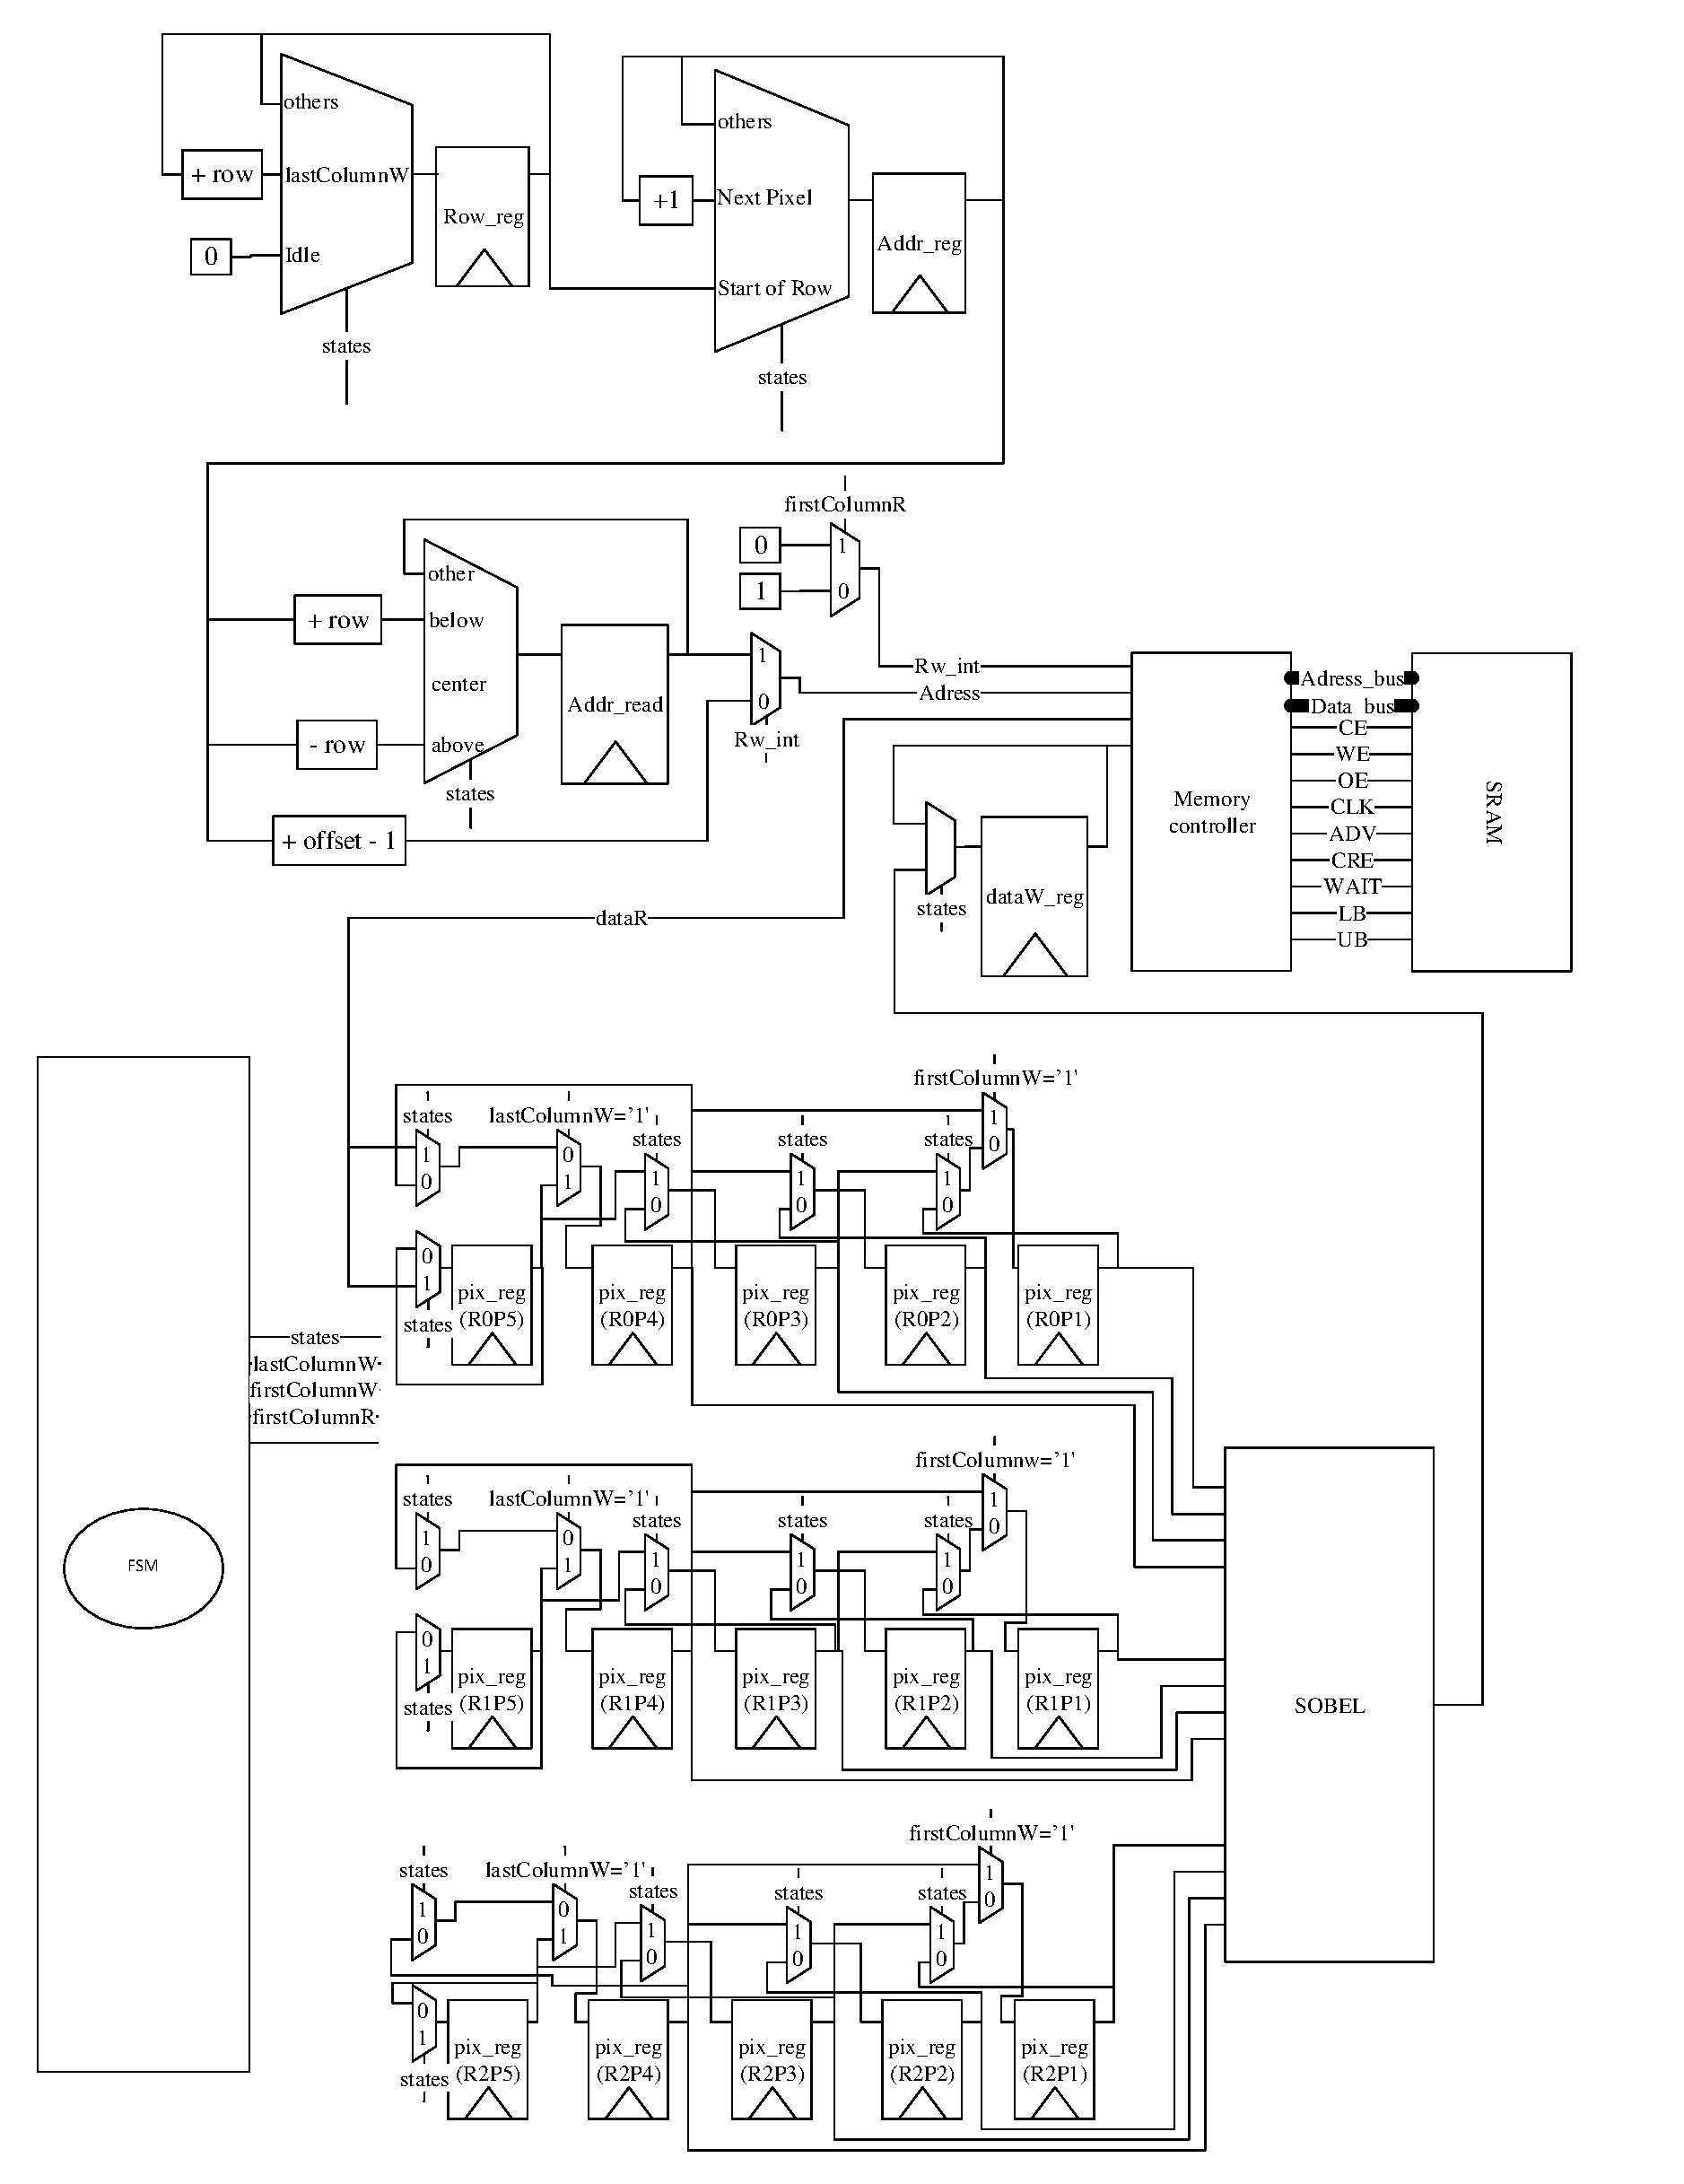
\includegraphics[width=1 \textwidth]{Block_diagram_detiled.pdf}
	\caption{Complete block diagram of the acc.vhdl code}
	\label{fig:block_acc}
\end{figure}